The Analog Devices AD5678-2 was chosen to be the DAC on the Electrophysiology Interface board because of previous experience with the device in the Neurobiology Engineering Laboratory~\cite{BatzerCorsiCrampton}.  The design for the circuit shown in Figure~\ref{fig:DAC} is based on a breadboarded prototype circuit~\cite{BatzerCorsiCrampton} and recommendations in the device data sheet~\cite{AD5678ds}.

\begin{figure}[H]
	\centering 
		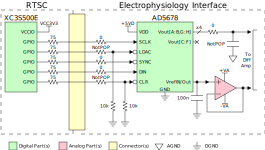
\includegraphics{./figures/StimAmp} 
	\caption{FPGA connections to the DAC\label{fig:DAC}}
\end{figure}

Signals from the Xilinx\textsuperscript{\textregistered} XC3S500E FPGA on the RTSC board are routed through the Hirose FX2 connector to the Electrophysiology Interface board and the 40-pin test header, finally going through a $0\unit{\Omega}$ resistor before being routed to the digital control pins of the AD5678.  The four 16-bit DAC analog outputs are routed to the Differential Output Amplifier circuits through a resistor that may be used, in concert with a capacitor, to implement an RC-type low pass filter.  The four 12-bit DAC outputs are left unconnected.  The FPGA configures the AD5678 to use its internal voltage reference for DAC operations, and thus, the Vref pin acts as the output of the internal voltage reference.  A 100nF capacitor is placed between the Vref pin and ground to stabilize the reference output~\cite{AD5678ds}, and the reference output voltage is used in the Differential Output Amplifier circuit, which requires the use of a buffer amplifier~\cite{AD5678ds}.  A description of each digital control pin is in Table~\ref{tab:AD5678Pins}.

\renewcommand{\arraystretch}{1.3}
\begin{table}[h]
\centering
\begin{tabular}{|l|p{4in}|}
\hline
Pin	& Function\\
\hline
$\overline{\mathrm{SYNC}}$	& Active low synchronization signal for input data, similar to SPI CS\\
\hline
DIN	& Serial data input\\
\hline
SCLK	& Serial clock input\\
\hline
$\overline{\mathrm{LDAC}}$	& Updates outputs simultaneously on a low pulse, it may be tied low if unused\\
\hline
$\overline{\mathrm{CLR}}$	& Falling edge triggered clear input that can set all the outputs to zero, mid-scale, or full-scale (default zero), pull down resistor keeps this from being noise triggered if unused\\
\hline
\end{tabular}
\caption{AD5678 Digital Pin Functions~\cite{AD5678ds}\label{tab:AD5678Pins} }

\end{table}
\renewcommand{\arraystretch}{1.0}

$\overline{\mathrm{SYNC}}$, DIN, and SCLK are mandatory signals for executing commands and loading data into the DAC.  The signals are compatible with SPI\textsuperscript{\textregistered}, QSPI\textsuperscript{TM}, MICROWIRE\textsuperscript{TM}, and DSP interface standards~\cite{AD5678ds}.  The $\overline{\mathrm{LDAC}}$ and $\overline{\mathrm{CLR}}$ signals provide additional functionality that is not used in the current version of the FPGA configuration.  Thus, the $0\unit{\Omega}$ resistors are not populated on the Electrophysiology Interface board, allowing the FPGA's GPIO pins to be accessed at the test header and used for other purposes if needed, and the DAC pins are pulled to ground through $10\unit{k\Omega}$ resistors to keep the inputs at a known state that will not affect the operation of the DAC.

The AD5678 contains a power-on reset circuit that sets the DAC outputs to 0V upon power up, which due to the Differential Output Amplifier may yield a significant voltage across the stimulation electrodes, which may be incompatible with the biological setup~\cite{AD5678ds}.  Therefore, upon power-up, the FPGA should immediately write DAC outputs or set the Clear Code Register and pulse the $\overline{\mathrm{CLR}}$ signal to set the DAC outputs to a value that will yield a voltage across the stimulation electrodes that is compatible with the experimental setup.  $\overline{\mathrm{CLR}}$ is a falling edge triggered signal that can also be used to asynchronously set all of the outputs to the state defined in the Clear Code Register of the AD5678~\cite{AD5678ds}.
